% !TeX spellcheck = en_GB
%-------------------------------------------------------------------------------
% File: simulation.tex
%       Vehicle ADVISE project documentation.
%
% Author: Yuri Mazzuoli, Francesco Iemma, Marco Pinna
%         Created on 30/06/2021
%-------------------------------------------------------------------------------
\chapter{Simulation}\label{ch:simulation}
\section{General Results}
We decide to simulate 200 units of time (200h) with Mobius in order to evaluate each attacker results for 
different configuration of mitigations. We obtain those general results:\\
\begin{itemize}
    \item the \textbf{Hacker} will always try to achieve the most remunerative goals, despite the
        possibility to be discovered; 
    \item the \textbf{Physical intruder} will try to achieve only the most remunerative goal, and will
        ignore others because of the high probability of being discovered (risk-reward ratio is too low)
    \item the \textbf{Insider} has the same behaviour of the Physical intruder, but for him the probability
        to reach the goal increases faster because his attack path has higher success probability.
\end{itemize}
\newpage
\section{Hacker Attacks}
\subsection*{DoS}
When no mitigation are applied, the Hacker will rarely try to obtain a DoS, but he will commit himself
on other attacks in order to obtain high reward goals. Introducing \textbf{CodeObfuscation}, binary reversing
become harder to complete with success, leading to a probability of reach DoS near to 0.\\
Increasing the firewall sensitivity will indeed increase the probability for the hacker to reach the DoS,
because he will give up on trying to reach other goals, focusing only on this one.
\begin{figure}[H]
    \begin{center}
        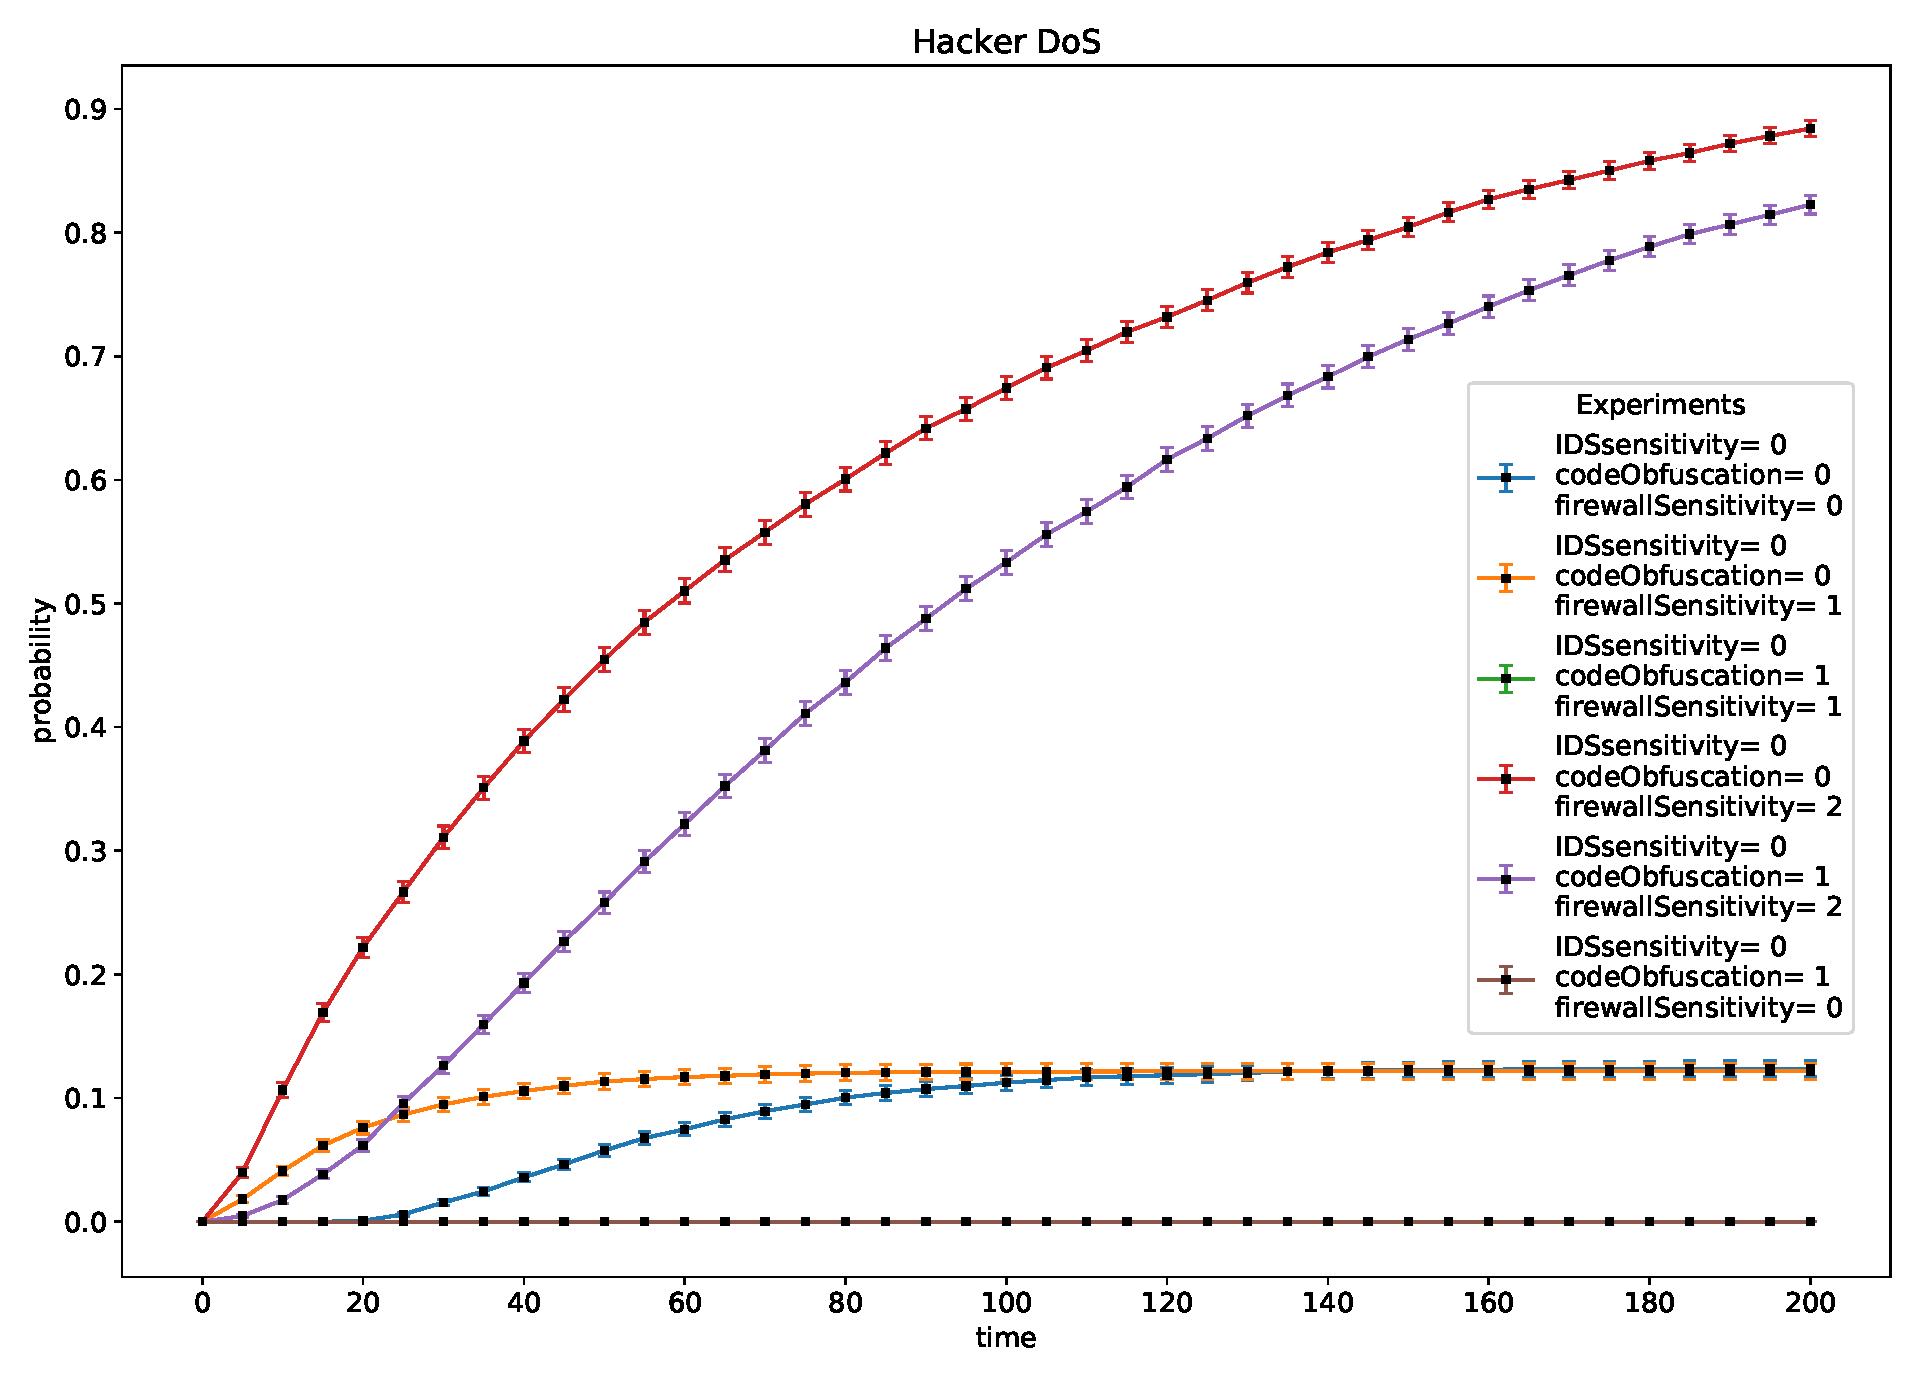
\includegraphics[scale=0.45]{img/Hacker_DoS.pdf}
    \end{center}
    \caption{Hacker DoS}
    \label{fig:Hacker_DoS}
    \vspace*{-0.8cm}
\end{figure}
\newpage
\subsection*{Data Breach and Vehicle Undesidered Behaviour}
When no mitigation are applied, the Hacker will reach those goals pretty fast. Introducing \textbf{CodeObfuscation}
will slow him down, but increasing \textbf{Firewall Sensitivity} we are able to reduce his will to reach them
until he will give up. 
\begin{figure}[H]
    \begin{center}
        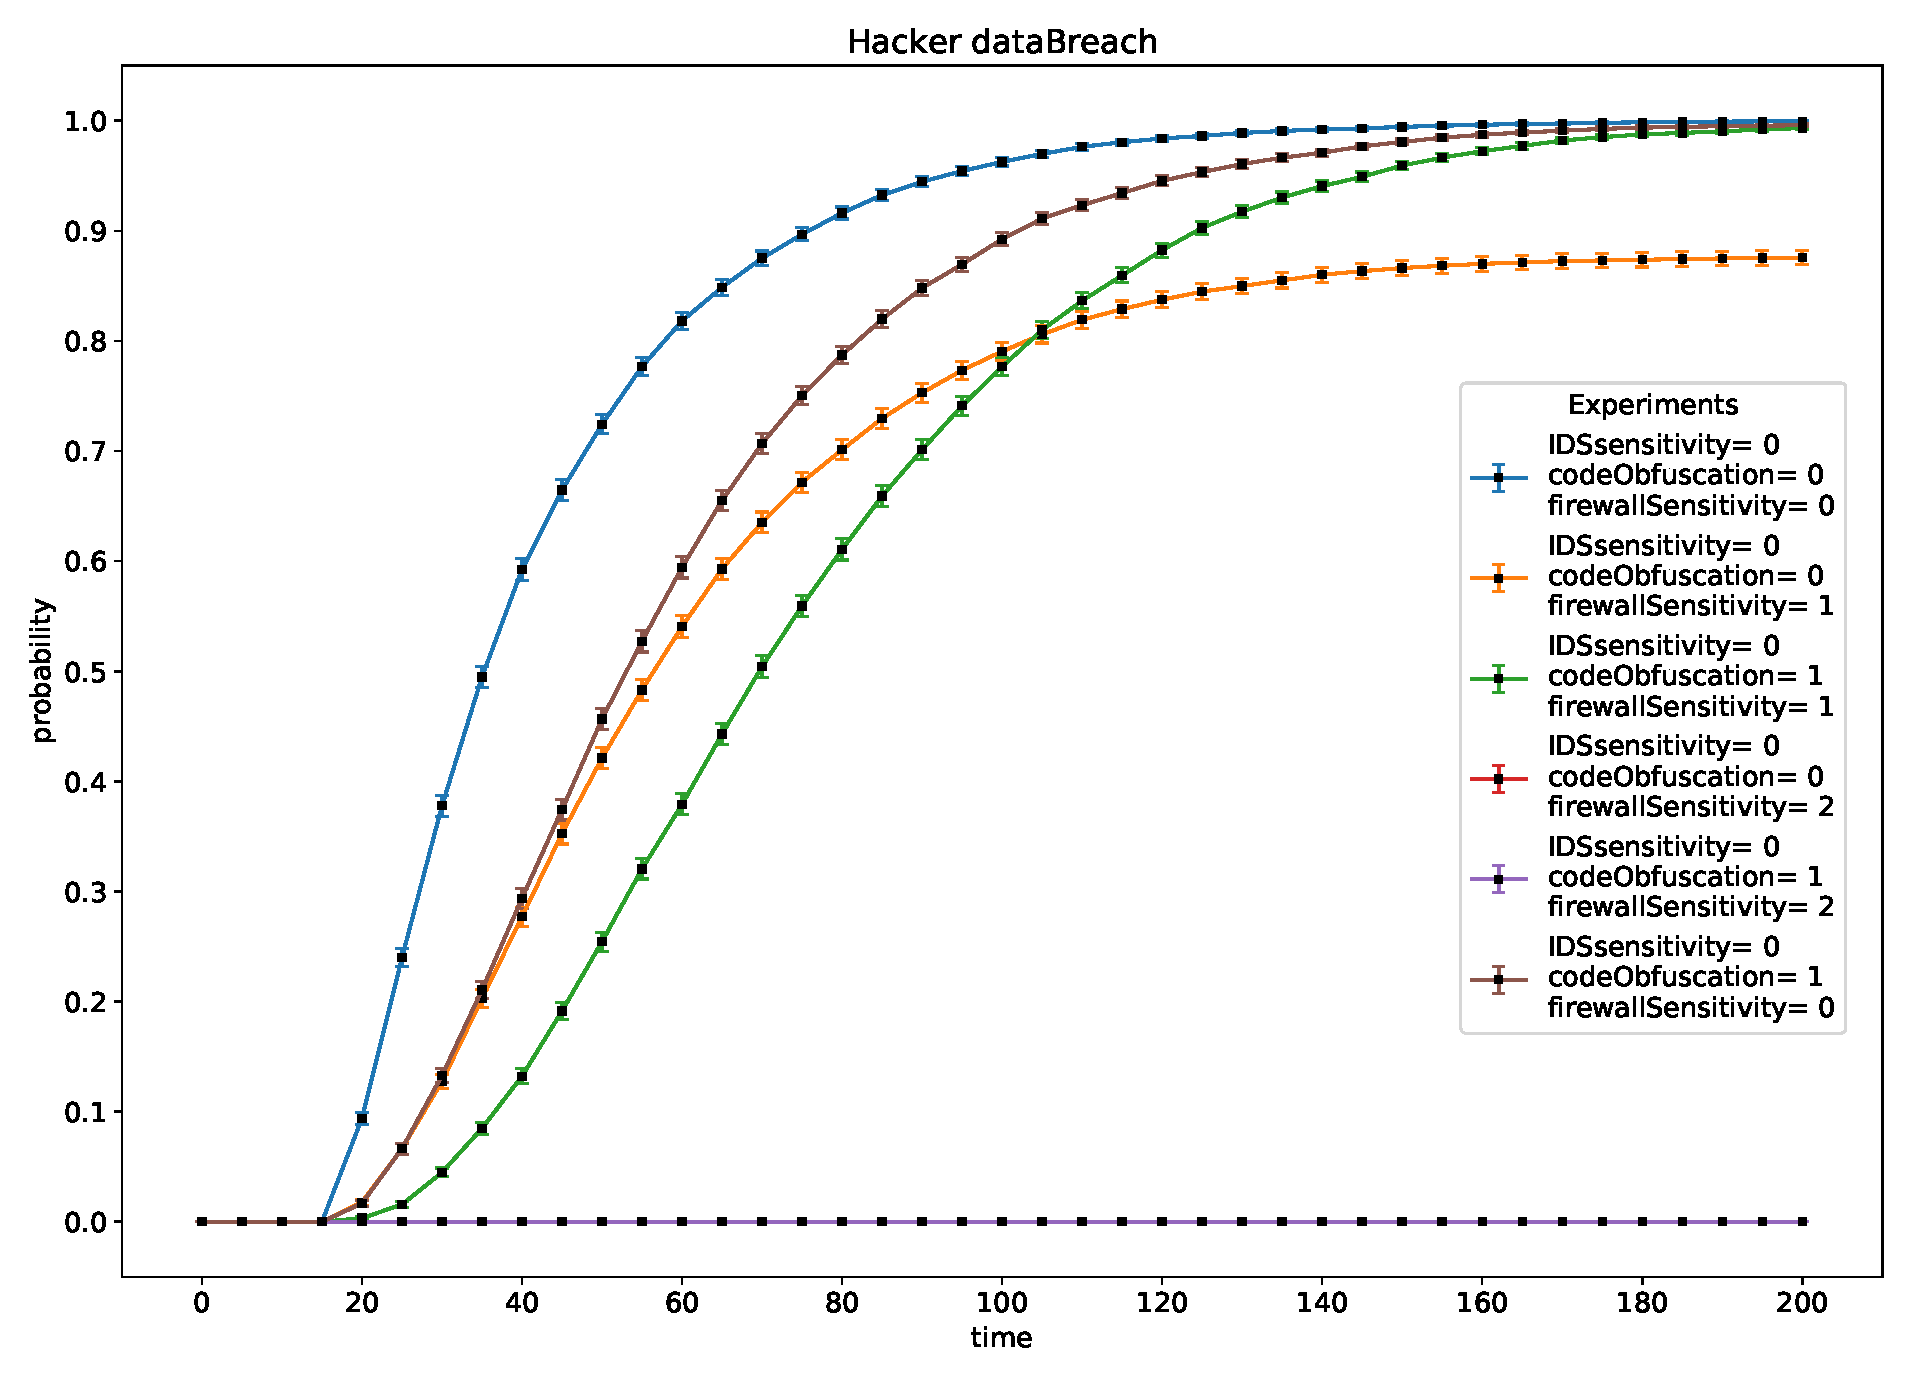
\includegraphics[scale=0.4]{img/Hacker_dataBreach.pdf}
        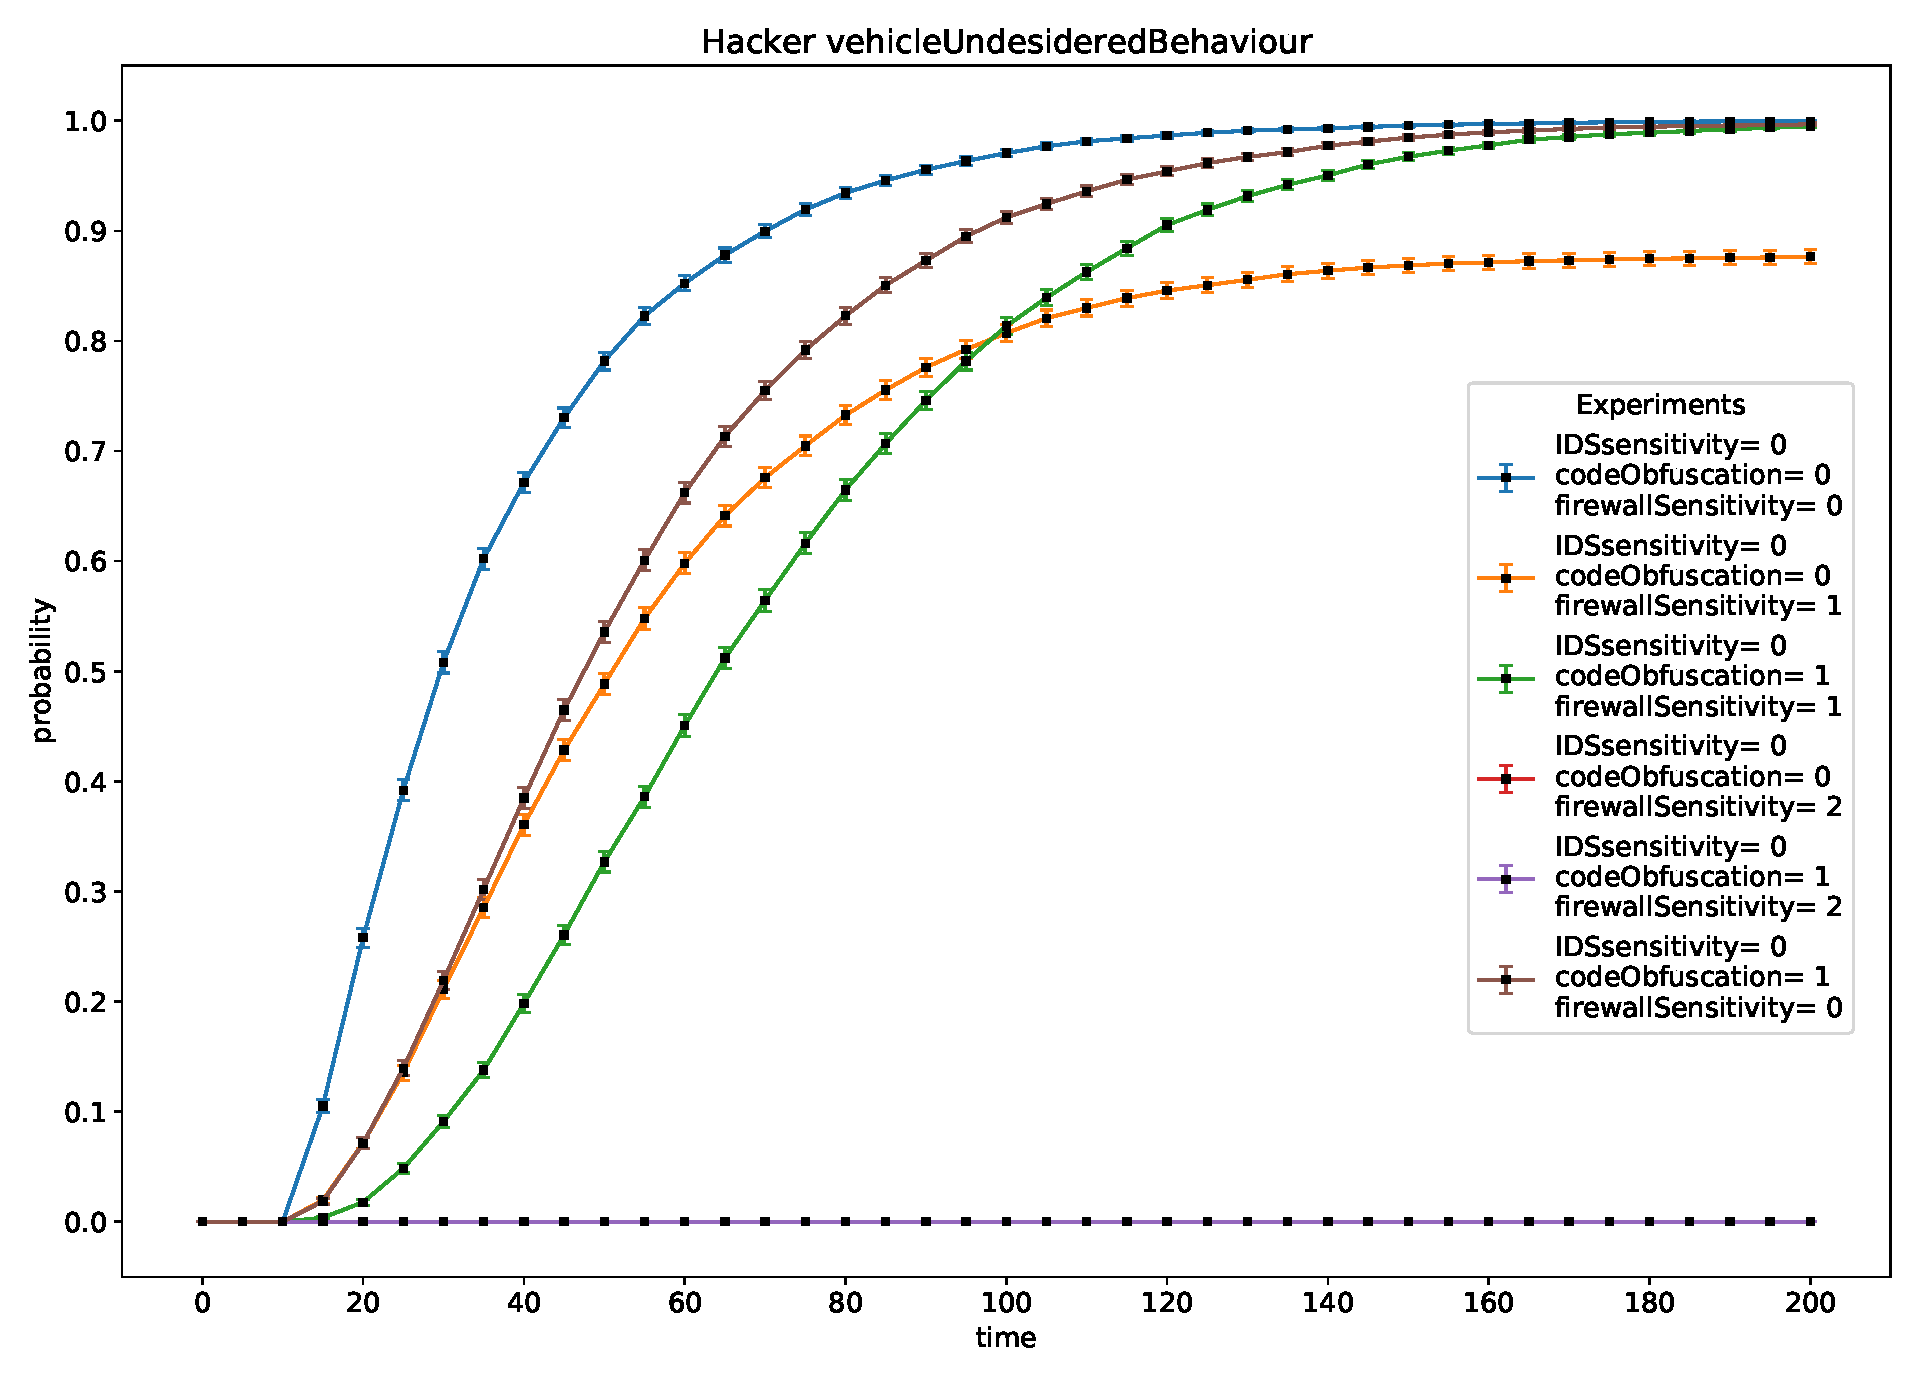
\includegraphics[scale=0.4]{img/Hacker_vOB.pdf}
    \end{center}
    \caption{Hacker Data Breach and Vehicle Undesidered Behaviour}
    \label{fig:Hacker_dataBreach}
    \vspace*{-2cm}
\end{figure}
\section{Physical Intruder and Insider Attacks}

\subsection*{Vehicle Undesidered Behaviour}
When no mitigation are applied, both attackers will reach this goal pretty fast. Increasing 
\textbf{Intrusion Detection System Sensitivity}, we are able to reduce their will to reach the goal
until they will give up, because the probability to be discovered will be to high.
\begin{figure}[H]
    \begin{center}
        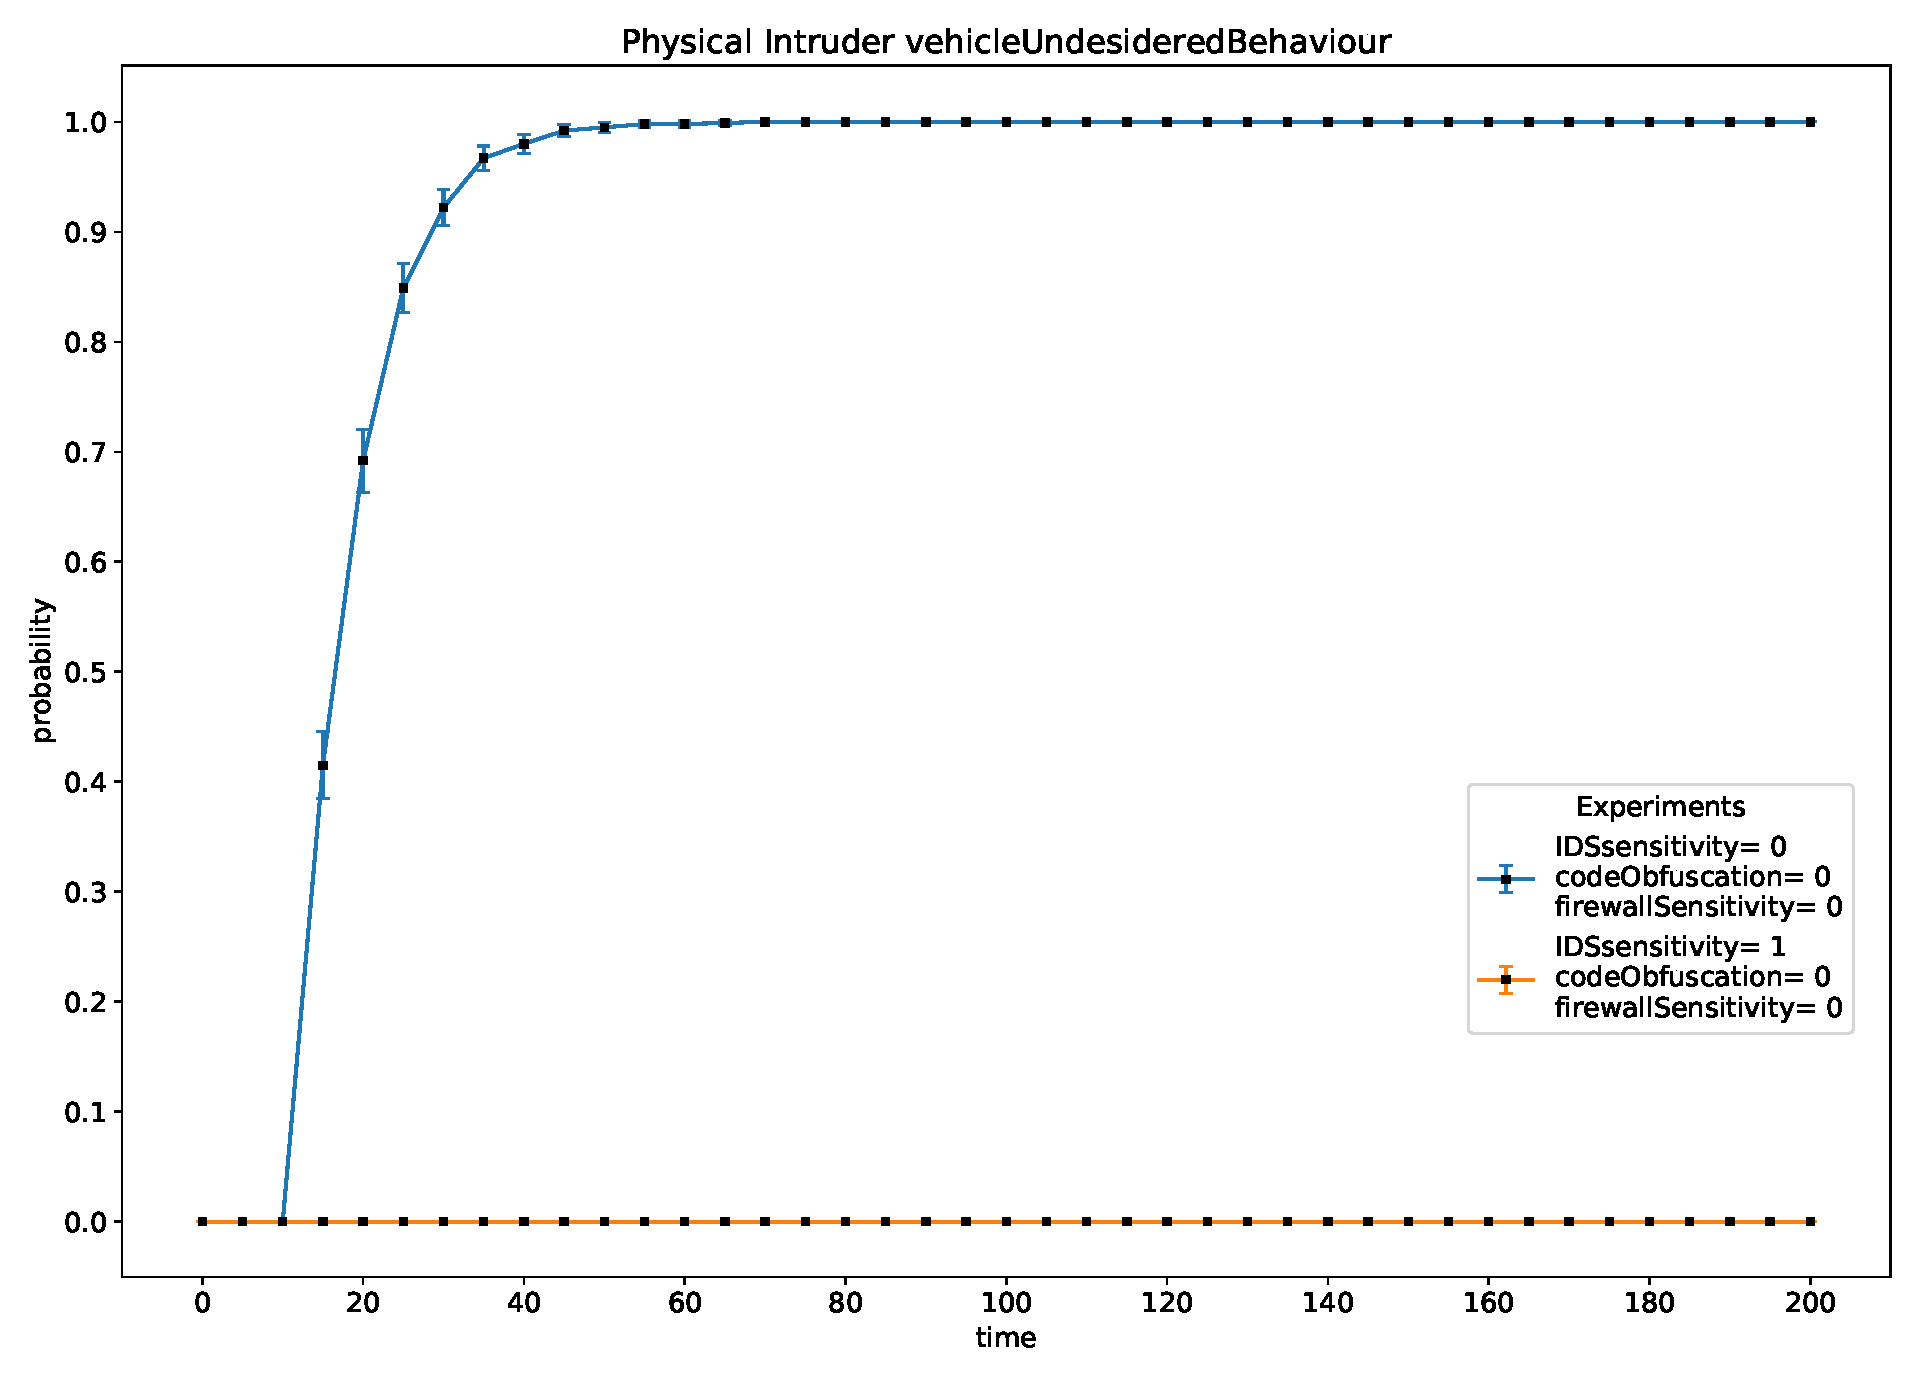
\includegraphics[scale=0.4]{img/Physical_vOB.pdf}
        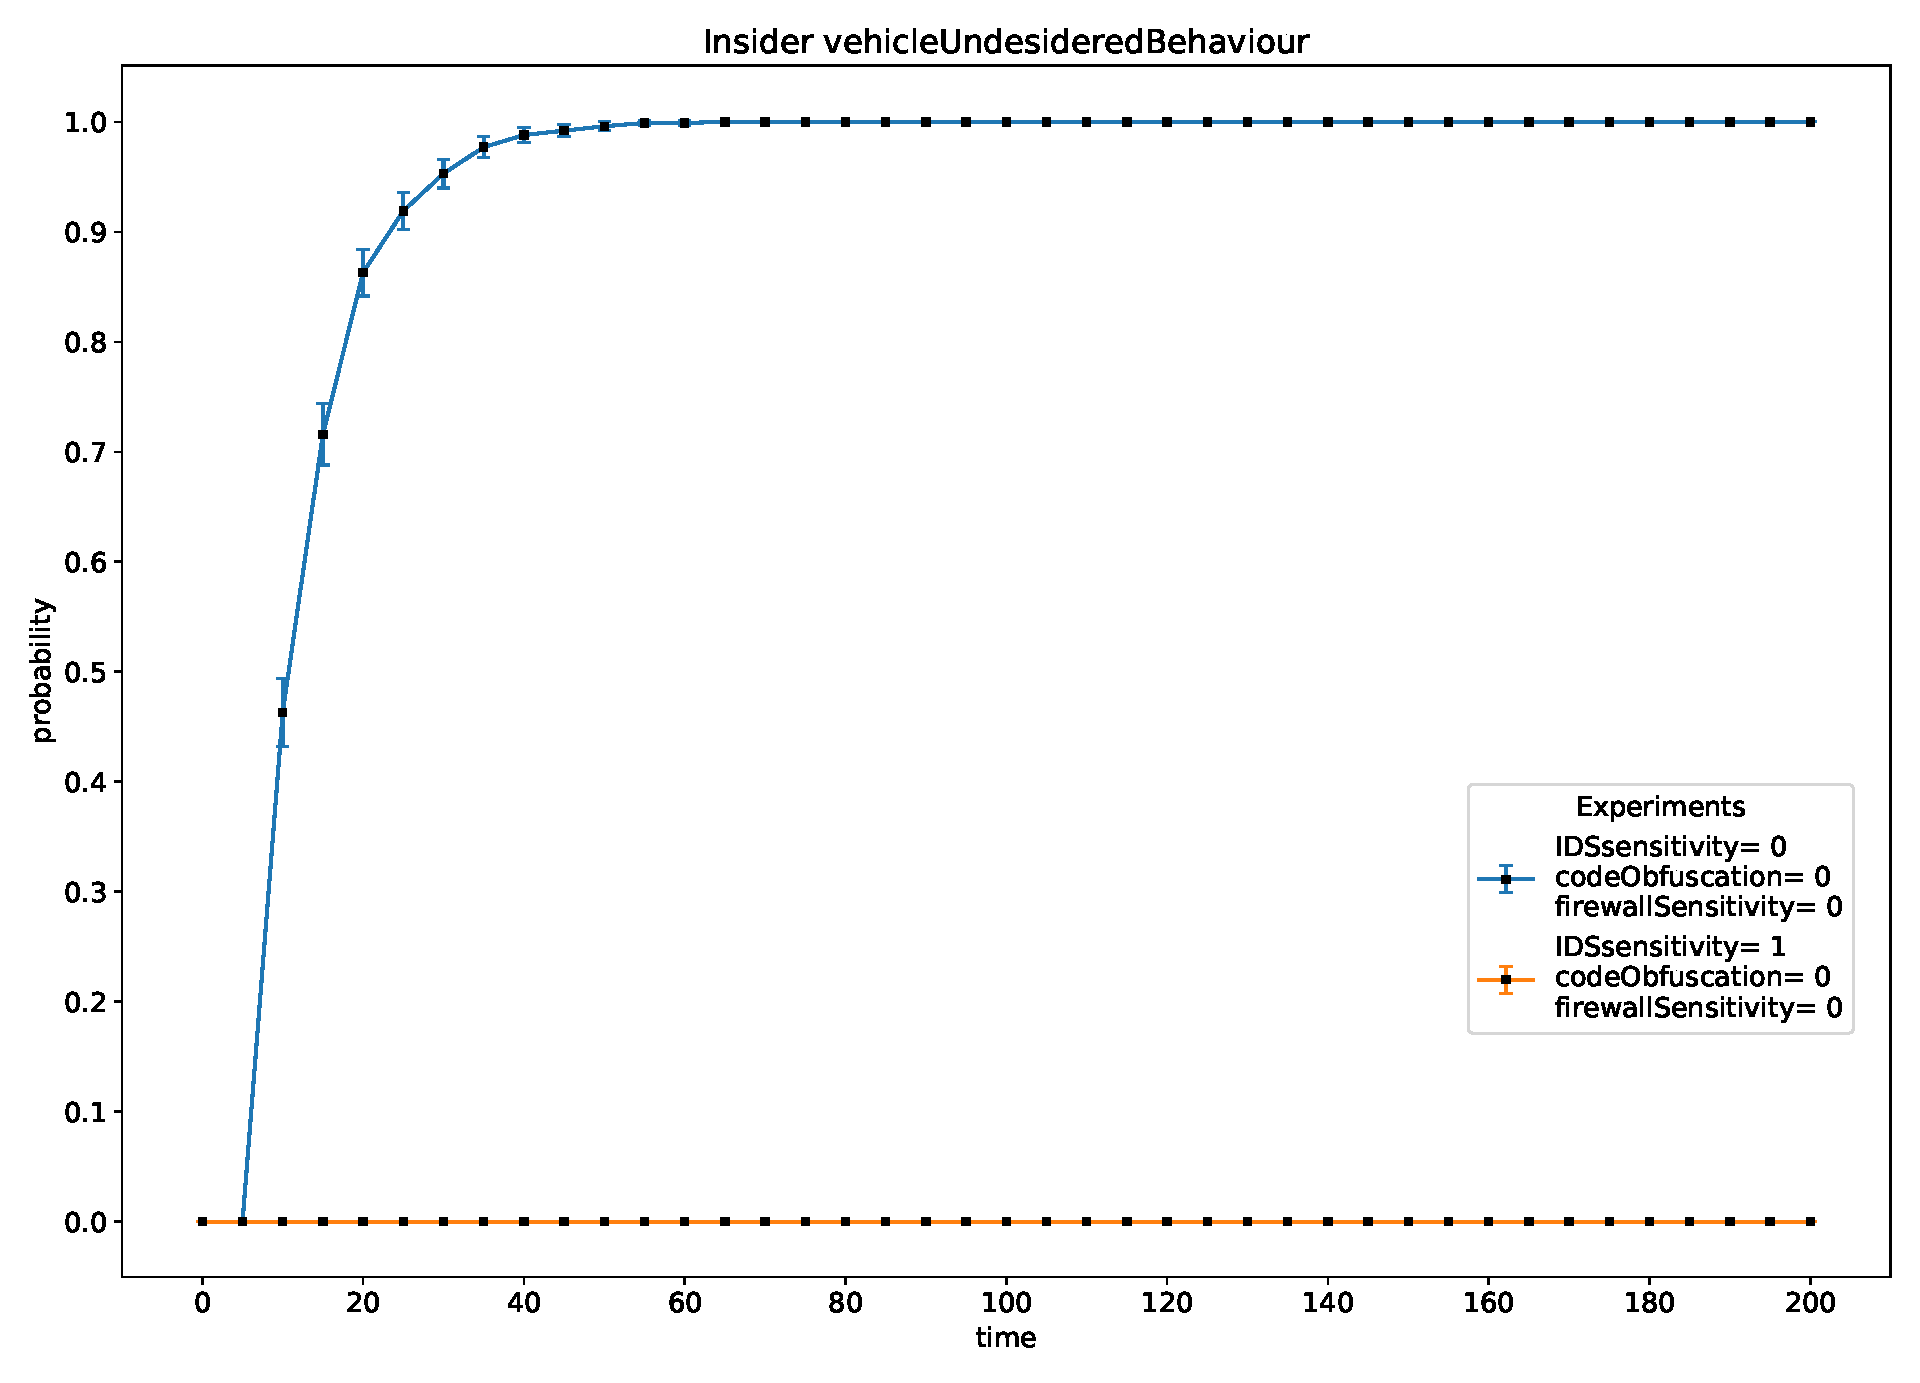
\includegraphics[scale=0.4]{img/Insider_vOB.pdf}
    \end{center}
    \caption{Physical intruder and Insider Vehicle Undesidered Behaviou}
    \label{fig:P_I_vob}
    \vspace*{-3cm}
\end{figure}

\noindent It is important to underline that in the case of insider attacker the time needed to achieve an high probability is lesser w.r.t. the one needed for a physical intruder, since the two attacker follows different path and the one of the physical intruder is longer and require more time.

\section{Conclusion}
\noindent At the end of our analysis we can infer that is a very good idea to invest in an high reliable and effective \textbf{Firewall} in order to discourage attacks from the hacker, furthermore also IDS and code obfuscation techniques are good countermeasures.

\noindent Thus implementing this mitigations causes an improvement in the security of the overall system.
